
CMake builds the solution in three stages – configuration, generation, and running the build tool. Generally, we have all the required data during the configuration stage. But every once in a while, we encounter the chicken and the egg problem. Take an example from the previous section – a target needs to know the path of a binary artifact of another target. But that information is only available after all the list files are parsed and the configuration stage is complete.

How do we deal with that kind of problem? We could create a placeholder for that information and postpone its evaluation to the next stage – the generation stage.

This is what generator expressions (sometimes called genexes) do. They are built around target properties such as LINK\_LIBRARIES, INCLUDE\_DIRECTORIES, COMPILE\_DEFINITIONS, propagated properties, and many others, but not all. They follow rules similar to conditional statements and variable evaluation.

It's worth noting that expressions are generally evaluated in the context of the target using the expression (unless explicitly stated otherwise).

\begin{tcolorbox}[colback=blue!5!white,colframe=blue!75!black,title=Important Note]
Generator expressions will be evaluated at the generation stage (when the configuration is complete and the buildsystem is created), which means that you can't capture their output into a variable and print it to the console very easily. To debug them, you can use either of these methods: 

\begin{itemize}
\item 
Write it to a file (this specific version of the file() command supports generator expressions): \begin{lstlisting}[style=styleCMake]
file(GENERATE OUTPUT filename CONTENT "$<...>")
\end{lstlisting}

\item 
Add a custom target and build it explicitly from the command line: 
\begin{lstlisting}[style=styleCMake]
custom_target(gendbg COMMAND ${CMAKE_COMMAND} -E echo "$<...>")
\end{lstlisting}
\end{itemize}
\end{tcolorbox}

\subsubsubsection{4.4.1\hspace{0.2cm}General syntax}

Let's take the simplest possible example:

\begin{lstlisting}[style=styleCMake]
target_compile_definitions(foo PUBLIC
	BAR=$<TARGET_FILE:foo>)
\end{lstlisting}

The preceding command adds a -D definition flag to the compiler's arguments (ignore PUBLIC for now) that sets the BAR preprocessor definition to the path of the binary artifact of the foo target.

How is the generator expression formed?

\begin{center}
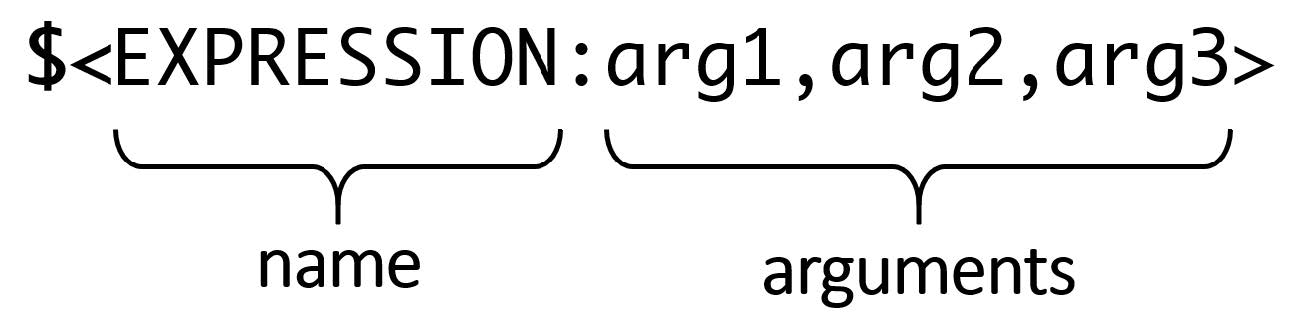
\includegraphics[width=0.5\textwidth]{content/2/chapter4/images/4.jpg}\\
Figure 4.4 – The syntax of a generator expression
\end{center}

As you can see in Figure 4.4, the structure seems fairly simple and readable:

\begin{itemize}
\item 
Open with a dollar and a bracket (\$<)

\item 
Add the EXPRESSION name

\item 
If an expression requires arguments, add a colon (:) and provide the arg1, arg2, and arg3 values, separated with a comma (,).

\item 
Close the expression with >.
\end{itemize}

There are even expressions that do not require any arguments, such as \$<PLATFORM\_ID>. However, generator expressions can quickly become very confusing and complicated when using their more advanced features.

\hspace*{\fill} \\ %插入空行
\noindent
\textbf{Nesting}

Let's start with the ability to pass a general expression as an argument to another expression or, in other words, general expression nesting:

\begin{lstlisting}[style=styleCMake]
$<UPPER_CASE:$<PLATFORM_ID>>
\end{lstlisting}

This isn't a very complex example, but it's easy to imagine what happens when we increase nesting levels and work with commands using multiple arguments.

As if that's not enough, you can technically add a variable expansion to this mix:

\begin{lstlisting}[style=styleCMake]
$<UPPER_CASE:${my_variable}>
\end{lstlisting}

A variable will be expanded at the configuration stage and a generation expression at the generation stage. There are some rare uses for this feature, but I strongly recommend avoiding it.

\hspace*{\fill} \\ %插入空行
\noindent
\textbf{Conditional expressions}

Boolean logic is supported in generator expressions. It's a great feature, but for legacy reasons, its syntax is inconsistent and can be hard to read. It's available in two forms. The first form supports both happy and sad paths:

\begin{lstlisting}[style=styleCMake]
$<IF:condition,true_string,false_string>
\end{lstlisting}

The syntax here is aligned with all other expressions and, like all expressions, nesting is allowed. So, you can replace any of the arguments with another expression and produce some very complex evaluations – you can even nest one condition in another. This form requires exactly three arguments, so we can't omit anything. Our best option to skip a value in case of an unmet condition is the following:

\begin{lstlisting}[style=styleCMake]
$<IF:condition,true_string,>
\end{lstlisting}

The second form is a shorthand for the preceding; it will only expand to a string if the condition is met:

\begin{lstlisting}[style=styleCMake]
$<condition:true_string >
\end{lstlisting}

As you can see, it breaks the convention of providing the EXPRESSION name as the first token. I assume that the intention here was to shorten the expression and skip those precious three characters, but the outcome can be really hard to rationalize. Here's one example from the CMake documentation:

\begin{lstlisting}[style=styleCMake]
$<$<AND:$<COMPILE_LANGUAGE:CXX>,$<CXX_COMPILER_ID:AppleClan
	g,Clang>>:COMPILING_CXX_WITH_CLANG>
\end{lstlisting}

I wish the syntax was aligned with conditions for the regular IF command, but sadly that's not the case.

\subsubsubsection{4.4.2\hspace{0.2cm}Types of evaluation}

Generator expressions are evaluated to one of two types – Boolean or string. Boolean is represented by 1 (true) and 0 (false). Everything else is just a string.

It's important to remember that nested expressions passed as conditions in conditional expressions are explicitly required to evaluate to Boolean.

There's an explicit logical operator to convert strings to Boolean, but Boolean types can be converted to strings implicitly.

Now that we know the basic syntax, let's take a look at what we can do with it.

\hspace*{\fill} \\ %插入空行
\noindent
\textbf{Evaluation to Boolean}

We started discussing conditional expressions in the previous section. I want to get the whole concept covered right off the bat so that there's no need to return to it later. There are three categories of expressions that get evaluated to Boolean.

\hspace*{\fill} \\ %插入空行
\noindent
\textbf{Logical operators}

There are four logical operators:

\begin{itemize}
\item 
\begin{lstlisting}[style=styleCMake]
$<NOT:arg> 
\end{lstlisting}

negates the Boolean argument.

\item 
\begin{lstlisting}[style=styleCMake]
$<AND:arg1,arg2,arg3...> 
\end{lstlisting}

returns 1 if all the arguments are 1.

\item 
\begin{lstlisting}[style=styleCMake]
$<OR:arg1,arg2,arg3...> 
# returns 1 if any of the arguments is 1.
\end{lstlisting}

\item 
\begin{lstlisting}[style=styleCMake]
$<BOOL:string_arg> 
\end{lstlisting}

converts arguments from a string to a Boolean type.
\end{itemize}

String conversion will evaluate to 1 if none of these conditions are met:

\begin{itemize}
\item 
The string is empty.

\item 
The string is a case-insensitive equivalent of 0, FALSE, OFF, N, NO, IGNORE, or NOTFOUND.

\item 
The string ends in the -NOTFOUND suffix (case-sensitive).
\end{itemize}

\hspace*{\fill} \\ %插入空行
\noindent
\textbf{String comparison}

Comparisons will evaluate to 1 if their condition is met and 0 otherwise:

\begin{itemize}
\item 
\begin{lstlisting}[style=styleCMake]
$<STREQUAL:arg1,arg2> 
\end{lstlisting}

is a case-sensitive string comparison.

\item 
\begin{lstlisting}[style=styleCMake]
$<EQUAL:arg1,arg2> 
\end{lstlisting}

converts a string to a number and compares equality.

\item 
\begin{lstlisting}[style=styleCMake]
$<IN_LIST:arg,list> 
\end{lstlisting}

checks whether the arg element is in the list list (case-sensitive).

\item 
\begin{lstlisting}[style=styleCMake]
$<VERSION_EQUAL:v1,v2>, $<VERSION_LESS:v1,v2>,
$<VERSION_GREATER:v1,v2>, $<VERSION_LESS_EQUAL:v1,v2>,
$<VERSION_GREATER_EQUAL:v1,v2> 
\end{lstlisting}
are component-wise version comparisons.
\end{itemize}

\hspace*{\fill} \\ %插入空行
\noindent
\textbf{Variable queries}

There are plenty of variables that contain Boolean-typed values. They also will evaluate to 1 if their condition is met and 0 otherwise.

There is one simple query:

\begin{itemize}
\item 
\begin{lstlisting}[style=styleCMake]
$<TARGET_EXISTS:arg> 
\end{lstlisting}
does the arg target exist?
\end{itemize}

There are multiple queries scanning passed arguments for a specific value:

\begin{itemize}
\item 
\begin{lstlisting}[style=styleCMake]
$<CONFIG:args>
\end{lstlisting}
is the current config (Debug, Release, and so on) in args (case-insensitive).

\item 
\begin{lstlisting}[style=styleCMake]
$<PLATFORM_ID:args>
\end{lstlisting}
is the current platform ID in args.

\item 
\begin{lstlisting}[style=styleCMake]
$<LANG_COMPILER_ID:args>
\end{lstlisting}
is CMake's LANG compiler ID in args, where LANG is one of C, CXX, CUDA, OBJC, OBJCXX, Fortran, or ISPC.

\item 
\begin{lstlisting}[style=styleCMake]
$<LANG_COMPILER_VERSION:args>
\end{lstlisting}
is the CMake's LANG compiler version in args, where LANG is one of C, CXX, CUDA, OBJC, OBJCXX, Fortran, or ISPC.

\item 
\begin{lstlisting}[style=styleCMake]
$<COMPILE_FEATURES:features>
\end{lstlisting}
will return true if features is supported by the compiler for this target.

\item 
\begin{lstlisting}[style=styleCMake]
$<COMPILE_LANG_AND_ID:lang,compiler_id1,compiler_id2...>
\end{lstlisting}
is the language of this lang target and is the compiler used for this target present in the compiler\_ids list. This expression is useful to specify details of a configuration for specific compilers:

\begin{lstlisting}[style=styleCMake]
target_compile_definitions(myapp PRIVATE
	$<$<COMPILE_LANG_AND_ID:CXX,AppleClang,Clang>:CXX_CLANG>
	$<$<COMPILE_LANG_AND_ID:CXX,Intel>:CXX_INTEL>
	$<$<COMPILE_LANG_AND_ID:C,Clang>:C_CLANG>
)
\end{lstlisting}

In the preceding example, if we compile the CXX compiler with AppleClang or Clang, the -DCXX\_CLANG definition will be set. For the CXX compiler from Intel, the -DCXX\_INTEL definition flag will be set. Lastly, for the C and Clang compiler, we'll get a -DC\_CLANG definition.

\item 
\begin{lstlisting}[style=styleCMake]
$<COMPILE_LANGUAGE:args>
\end{lstlisting}

if a language is used for the compilation of this target in args. This can be used to provide language-specific flags to the compiler:

\begin{lstlisting}[style=styleCMake]
target_compile_options(myapp
	PRIVATE $<$<COMPILE_LANGUAGE:CXX>:-fno-exceptions>
)
\end{lstlisting}

If we compile CXX, the compiler will use the -fno-exceptions flag

\item 
\begin{lstlisting}[style=styleCMake]
$<LINK_LANG_AND_ID:lang,compiler_id1,compiler_id2...>
\end{lstlisting}
works similarly to COMPILE\_LANG\_AND\_ID but checks the language used for the link step instead. Use this expression to specify link libraries, link options, link directories, and link dependencies of a particular language and a linker combination in a target.

\item 
\begin{lstlisting}[style=styleCMake]
$<LINK_LANGUAGE:args>
\end{lstlisting}

is the language used for the link step in args.
\end{itemize}

\hspace*{\fill} \\ %插入空行
\noindent
\textbf{Evaluation to a string}

There are plenty of expressions that get evaluated to a string. We can output them directly to the placeholder of the target or consume as an argument to another expression. We already learned about one – conditional expression evaluates to a string. What else is available?

\hspace*{\fill} \\ %插入空行
\noindent
\textbf{Variable queries}

These expressions will evaluate to a specific value at the generation stage:

\begin{itemize}
\item 
\begin{lstlisting}[style=styleCMake]
$<CONFIG> 
\end{lstlisting}

the configuration (Debug and Release) name.

\item 
\begin{lstlisting}[style=styleCMake]
$<PLATFORM_ID>
\end{lstlisting}

the current system's CMake platform ID (Linux, Windows, or Darwin). We discussed platform in the previous chapter, in the Scoping the environment section.

\item 
\begin{lstlisting}[style=styleCMake]
$<LANG_COMPILER_ID> 
\end{lstlisting}

CMake's compiler ID of the LANG compiler used, where LANG is one of C, CXX, CUDA, OBJC, OBJCXX, Fortran, or ISPC.

\item 
\begin{lstlisting}[style=styleCMake]
$<LANG_COMPILER_VERSION> 
\end{lstlisting}

CMake's compiler version of the LANG compiler used, where LANG is one of C, CXX, CUDA, OBJC, OBJCXX, Fortran, or ISPC.

\item 
\begin{lstlisting}[style=styleCMake]
$<COMPILE_LANGUAGE>
\end{lstlisting}

the compiled language of source files when evaluating compile options.

\item 
\begin{lstlisting}[style=styleCMake]
$<LINK_LANGUAGE>
\end{lstlisting}

the link language of a target when evaluating link options.
\end{itemize}

\hspace*{\fill} \\ %插入空行
\noindent
\textbf{Target-dependent queries}

With the following queries, you can evaluate properties of an executable or library target. Note that since CMake 3.19, for most expressions querying a target in the context of another target no longer creates an automated dependency between these targets (as was happening before 3.19):

\begin{itemize}
\item 
\begin{lstlisting}[style=styleCMake]
$<TARGET_NAME_IF_EXISTS:target>
\end{lstlisting}

the target name of target if it exists; it is an empty string otherwise.

\item 
\begin{lstlisting}[style=styleCMake]
$<TARGET_FILE:target>
\end{lstlisting}

the full path to the target binary file.

\item 
\begin{lstlisting}[style=styleCMake]
$<TARGET_FILE_NAME:target>
\end{lstlisting}

the target filename.

\item 
\begin{lstlisting}[style=styleCMake]
$<TARGET_FILE_BASE_NAME:target>
\end{lstlisting}

the base name of target, or

\begin{lstlisting}[style=styleCMake]
$<TARGET_FILE_NAME:target>
\end{lstlisting}

without a prefix and suffix. For libmylib.so, the base name would be mylib.

\item 
\begin{lstlisting}[style=styleCMake]
$<TARGET_FILE_PREFIX:target> 
\end{lstlisting}

the prefix of the target filename (lib).

\item 
\begin{lstlisting}[style=styleCMake]
$<TARGET_FILE_SUFFIX:target>
\end{lstlisting}

the suffix (or extension) of the target filename (.so, .exe).

\item 
\begin{lstlisting}[style=styleCMake]
$<TARGET_FILE_DIR:target>
\end{lstlisting}

the directory of the target binary file

\item 
\begin{lstlisting}[style=styleCMake]
$<TARGET_LINKER_FILE:target>
\end{lstlisting}

the file used when linking to the target target. Usually, it is the library that target represents (.a, .lib, .so) on platforms with Dynamically Linked Libraries (DLL); for a shared library, it will be a .lib import library.

TARGET\_LINKER\_FILE offers the same family of expressions as the regular TARGET\_FILE expression:

\begin{lstlisting}[style=styleCMake]
$<TARGET_LINKER_FILE_NAME:target>, $<TARGET_LINKER_FILE_
BASE_NAME:target>, $<TARGET_LINKER_FILE_PREFIX:target>,
$<TARGET_LINKER_FILE_SUFFIX:target>,
$<TARGET_LINKER_FILE_DIR:target>
\end{lstlisting}

\item 
\begin{lstlisting}[style=styleCMake]
$<TARGET_SONAME_FILE:target>
\end{lstlisting}

the full path to a file with a soname(.so.3).

\item 
\begin{lstlisting}[style=styleCMake]
$<TARGET_SONAME_FILE_NAME:target>
\end{lstlisting}

the name of a file with a soname.

\item 
\begin{lstlisting}[style=styleCMake]
$<TARGET_SONAME_FILE_DIR:target> 
\end{lstlisting}

the directory of a file with a soname.

\item 
\begin{lstlisting}[style=styleCMake]
$<TARGET_PDB_FILE:target>
\end{lstlisting}

the full path to the linker generated program database file (.pdb) for target.

PDB files offer the same expressions as a regular TARGET\_FILE:

\begin{lstlisting}[style=styleCMake]
$<TARGET_PDB_FILE_BASE_NAME:target>, $<TARGET_PDB_FILE_NAME:target>,
$<TARGET_PDB_FILE_DIR:target>
\end{lstlisting}

\item 
\begin{lstlisting}[style=styleCMake]
$<TARGET_BUNDLE_DIR:target> 
\end{lstlisting}

the full path to the bundle (Apple–specific package) directory (my.app, my.framework, or my.bundle) for target.

\item 
\begin{lstlisting}[style=styleCMake]
$<TARGET_PROPERTY:target,prop>
\end{lstlisting}

the prop value for target.

\item 
\begin{lstlisting}[style=styleCMake]
$<TARGET_PROPERTY:prop>
\end{lstlisting}

the prop value for target for which the expression is being evaluated.

\item 
\begin{lstlisting}[style=styleCMake]
$<INSTALL_PREFIX> 
\end{lstlisting}

the install prefix when the target is exported with install(EXPORT) or when evaluated in INSTALL\_NAME\_DIR; otherwise, it is empty.

\end{itemize}

\hspace*{\fill} \\ %插入空行
\noindent
\textbf{Escaping}

On a rare occasion, you may need to pass a character to a generator expression that has a special meaning. To escape this behavior, use the following expressions:

\begin{itemize}
\item 
\begin{lstlisting}[style=styleCMake]
$<ANGLE-R>
\end{lstlisting}

a literal > symbol (which compares strings containing >)

\item 
\begin{lstlisting}[style=styleCMake]
$<COMMA>
\end{lstlisting}

a literal , symbol (which compares strings containing ,)

\item 
\begin{lstlisting}[style=styleCMake]
$<SEMICOLON>
\end{lstlisting}

a literal ; symbol (which prevents a list expansion on an argument with ;)
\end{itemize}

\hspace*{\fill} \\ %插入空行
\noindent
\textbf{String transformations}

Working with strings in the generator stage is possible with the following expressions:

\begin{itemize}
\item 
\begin{lstlisting}[style=styleCMake]
$<JOIN:list,d> 
\end{lstlisting}

join a semicolon-separated list using a d delimiter.

\item 
\begin{lstlisting}[style=styleCMake]
$<REMOVE_DUPLICATES:list>
\end{lstlisting}

remove duplicates without sorting list.

\item 
\begin{lstlisting}[style=styleCMake]
$<FILTER:list,INCLUDE|EXCLUDE,regex>
\end{lstlisting}

include/exclude items from a list using a regex regular expression.

\item 
\begin{lstlisting}[style=styleCMake]
$<LOWER_CASE:string>, $<UPPER_CASE:string>
\end{lstlisting}

convert the string to another case.

\item 
\begin{lstlisting}[style=styleCMake]
$<GENEX_EVAL:expr>
\end{lstlisting}

evaluate the expr string as a nested expression in the context of the current target. This is useful when an evaluation of a nested expression returns another expression (they aren't evaluated recursively).

\item 
\begin{lstlisting}[style=styleCMake]
$<TARGET_GENEX_EVAL:target,expr>
\end{lstlisting}

evaluate expr similarly to the GENEX\_EVAL transformation but in the context of target.
\end{itemize}

\hspace*{\fill} \\ %插入空行
\noindent
\textbf{Output-related expressions}

CMake documentation fails to provide a good explanation of what "output-related expressions" are. That leaves us a little lost; how are they related to output?

As per the v3.13 documentation (removed in newer revisions), "These expressions generate output, in some cases depending on an input." 

It turns out that they are a little bit of everything really. Some are a legacy version of the shorthand conditional expression. Others are just a string transformation expression that hadn't yet made its way into the other section.

The following expressions will return their first arguments if a specific condition is met and an empty string otherwise:

\begin{itemize}
\item 
\begin{lstlisting}[style=styleCMake]
$<LINK_ONLY:deps>
\end{lstlisting}

sets implicitly with target\_link\_libraries() to store PRIVATE deps link dependencies, which won't be propagated as usage requirements

\item 
\begin{lstlisting}[style=styleCMake]
$<INSTALL_INTERFACE:content>
\end{lstlisting}

returns content if used with install(EXPORT)

\item 
\begin{lstlisting}[style=styleCMake]
$<BUILD_INTERFACE:content> 
\end{lstlisting}

returns content if used with an export() command or by another target in the same buildsystem
\end{itemize}

The following output expressions will perform a string transformation on their arguments:

\begin{itemize}
\item 
\begin{lstlisting}[style=styleCMake]
$<MAKE_C_IDENTIFIER:input> 
\end{lstlisting}

converts to a C identifier following the same behavior as string(MAKE\_C\_IDENTIFIER).

\item 
\begin{lstlisting}[style=styleCMake]
$<SHELL_PATH:input>
\end{lstlisting}

converts an absolute path (or list of paths) to a shell path style matching the target OS. Slashes are converted to backslashes in Windows shells and drive letters are converted to POSIX paths in MSYS shells.
\end{itemize}

Finally, we have a stray variable query expression:

\begin{itemize}
\item 
\begin{lstlisting}[style=styleCMake]
$<TARGET_OBJECTS:target> 
\end{lstlisting}

returns a list of object files from a target object library
\end{itemize}

\subsubsubsection{4.4.3\hspace{0.2cm}Examples to try out}

Everything is easier to grasp when there's a good practical example to support the theory. Here are some of the uses for generator expressions:

\hspace*{\fill} \\ %插入空行
\noindent
\textbf{Build configurations}

In the first chapter, we discussed build type specifying which configuration we are building – Debug, Release, and so on. There may be cases where you'd like to act differently based on what kind of build you're making. A simple and easy way to do so is utilizing the \$<CONFIG> generator expression:

\begin{lstlisting}[style=styleCMake]
target_compile_options(tgt $<$<CONFIG:DEBUG>:-ginlinepoints>)
\end{lstlisting}

The preceding example checks whether the config equals DEBUG; if that's the case, the nested expression is evaluated to 1. The outer shorthand if expression then becomes true, and our -ginline-points debug flag gets added to the options.

\hspace*{\fill} \\ %插入空行
\noindent
\textbf{System-specific one-liners}

Generator expressions can also be used to compact verbose if commands into neat one-liners. Let's suppose we have the following code:

\begin{lstlisting}[style=styleCMake]
if (${CMAKE_SYSTEM_NAME} STREQUAL "Linux")
	target_compile_definitions(myProject PRIVATE LINUX=1)
endif()
\end{lstlisting}

It tells the compiler to add -DLINUX=1 to the arguments if this is the target system. While this isn't terribly long, it could be easily replaced with an elegant expression:

\begin{lstlisting}[style=styleCMake]
target_compile_definitions(myProject PRIVATE
	$<$<CMAKE_SYSTEM_NAME:LINUX>:LINUX=1>)
\end{lstlisting}

Such code works well, but there's a limit to how much you can pack into a generator expression until it becomes too hard to read. In that case, it's better to stick to the long conditional blocks.

\hspace*{\fill} \\ %插入空行
\noindent
\textbf{Interface libraries with compiler-specific flags}

Interface libraries, as we discussed earlier in this chapter, can be used to provide flags to match the compiler:

\begin{lstlisting}[style=styleCMake]
add_library(enable_rtti INTERFACE)
target_compile_options(enable_rtti INTERFACE
	$<$<OR:$<COMPILER_ID:GNU>,$<COMPILER_ID:Clang>>:-rtti>
)
\end{lstlisting}

Even in such a simple example, we can already see what happens when we nest too many generator expressions. Unfortunately, sometimes this is the only way to achieve the desired effect. Here's what happens:

\begin{itemize}
\item 
We check whether COMPILER\_ID is GNU; if that's the case, we evaluate OR to 1.

\item 
If it's not, we check whether COMPILER\_ID is Clang, and evaluate OR to 1. Otherwise, evaluate OR to 0

\item 
If OR is evaluated to 1, add -rtti to the enable\_rtti compile options. Otherwise, do nothing.
\end{itemize}

Next, we can link our libraries and executables with the enable\_rtti interface library. CMake will add the -rtti flag if a compiler supports it.

\hspace*{\fill} \\ %插入空行
\noindent
\textbf{Nested generator expressions}

Sometimes, it's not obvious what happens when we try to nest elements in a generator expression. We can debug the expressions by generating a test output to a debug file.

Let's try out a few things and see what happens:

\begin{lstlisting}[style=styleCMake]
# chapter04/04-genex/CMakeLists.txt (fragment)

set(myvar "small text")
set(myvar2 "small > text")

file(GENERATE OUTPUT nesting CONTENT
	"1 $<PLATFORM_ID>
	2 $<UPPER_CASE:$<PLATFORM_ID>>
	3 $<UPPER_CASE:hello world>
	4 $<UPPER_CASE:${myvar}>
	5 $<UPPER_CASE:${myvar2}>
")
\end{lstlisting}

The output is as follows:

\begin{tcblisting}{commandshell={}}
# cat nesting
1 Linux
  2 LINUX
  3 HELLO WORLD
  4 SMALL TEXT
  5 SMALL text>
\end{tcblisting}

This is how each line works:

\begin{enumerate}
\item 
The PLATFORM\_ID output value is regular case Linux.

\item 
The output from the nested value will get transformed correctly to uppercase LINUX.

\item 
We can transform plain strings.

\item 
We can transform the content of configuration-stage variables.

\item 
Variables will be interpolated first, and closing angle brackets (>) will be interpreted as part of the genex, in that only part of the string will get capitalized.
\end{enumerate}

In other words, be aware that the content of variables may affect the behavior of your genex expansions. If you need an angle bracket in a variable, use \$<ANGLE-R>.

\hspace*{\fill} \\ %插入空行
\noindent
\textbf{The difference between a conditional expression and the evaluation of BOOL operator}

Generator expressions can be a little confusing when it comes to evaluating Boolean types to strings. It is important to understand how they differ from regular conditional expressions, starting with an explicit IF keyword:

\begin{lstlisting}[style=styleCMake]
# chapter04/04-genex/CMakeLists.txt (fragment)

file(GENERATE OUTPUT boolean CONTENT
	"1 $<0:TRUE>
	2 $<0:TRUE,FALSE> (won't work)
	3 $<1:TRUE,FALSE>
	4 $<IF:0,TRUE,FALSE>
	5 $<IF:0,TRUE,>
")
\end{lstlisting}

This produces a file like this:

\begin{tcblisting}{commandshell={}}
# cat boolean
1
  2 (won't work)
  3 TRUE,FALSE 
  4 FALSE
  5
\end{tcblisting}

Let's examine the output for each line:

\begin{enumerate}
\item 
This is a Boolean expansion, where BOOL is 0; therefore, the TRUE string isn't written.

\item 
This is a typical mistake – the author intended to print TRUE or FALSE depending on the BOOL value, but since it is a Boolean false expansion as well, two arguments are treated as one and not printed.

\item 
This is the same mistake for a reversed value – it is a Boolean true expansion that has both arguments written in a single line.

\item 
This is a proper conditional expression starting with IF – it prints FALSE because the first argument is 0.

\item 
This is the incorrect usage of a conditional expression – when we don't need to write values for Boolean false, we should use the first form.
\end{enumerate}

Generator expressions are known for their convoluted syntax. The differences mentioned in this example can confuse even experienced builders. If in doubt, copy such an expression to another file and break it apart with added indentation and whitespace to understand it better.










